\Solution{2: MC Estimates and TD Learning}
\\

\noindent I started by implementing the \texttt{RandomWalk-v0} environment by subclassing the \texttt{gym.Env} class. The environment is a simple random walk with 7 states. The agent starts at the middle state and only moves left following the ``go-left'' policy. The agent terminates actions and receives a reward of $+1$ if it reaches the rightmost state and a reward of $0$ if it reaches the leftmost state. The agent receives a reward of $0$ on non-terminal states. The environment is completely stochastic and the agent has a probability of $0.5$ of moving left and right. The environment is working as expected, based on pygame observations and trajectory anaylsis.

In all the below test cases and scenarios a seed of $21$ is used. I have also added \texttt{CONFIG} dictionary at any code block which is producing an output to be able to change values and observe outputs.
\begin{enumerate}
    
    \item I created a function \texttt{generate\_episode\_trajectory(environment, config=None)} which takes in the \texttt{environment} and a \texttt{config} dictionary and returns a list of tuples of the form $(s, a, r, s^{\prime})$. I tested the function with the \texttt{RandomWalk-v0} environment and the trajectory is as expected. The trajectory is shown in the code block below.
    \begin{verbatim}
Episode Trajectory: [(3, 0, 0.0, 2), (2, 0, 0.0, 3), (3, 0, 0.0, 4), 
(4, 0, 0.0, 3), (3, 0, 0.0, 2), (2, 0, 0.0, 3), (3, 0, 0.0, 4), 
(4, 0, 0.0, 5), (5, 0, 1.0, 6)]
    \end{verbatim}
    
    \item I wrote a routine to decay the step size at every step/episode: \texttt{decay\_step\_size(initial\_value, final\_value, episode, max\_episode, decay\_type, decay\_stop=None)}. This routine returns $\alpha(e)$ which starts at \texttt{initial\_value} and ends at \texttt{final\_value} based on the \texttt{decay\_type}. I tested the function and the results are present in Figure \ref{fig:exp_step_size_decay} and Figure \ref{fig:linear_step_size_decay}. The step size is decaying as expected.
    \begin{figure}[h]
        \centering
        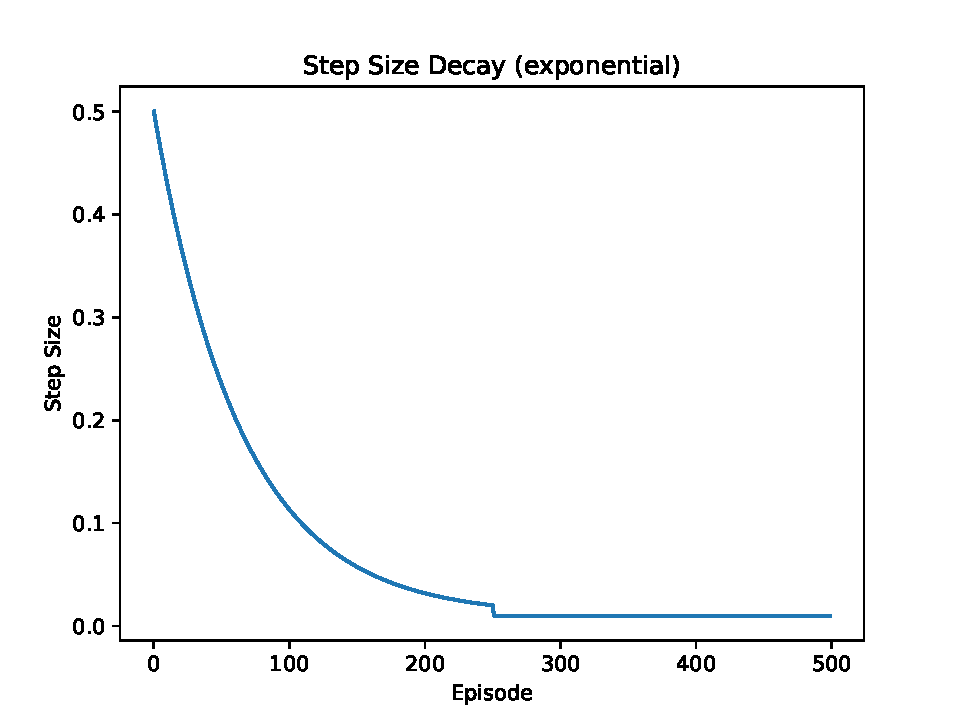
\includegraphics[width=0.8\textwidth]{images/mc_td/step_size_decay_exponential.pdf}
        \caption{Exponential decay of step size}
        \label{fig:exp_step_size_decay}
    \end{figure}
    \begin{figure}[h]
        \centering
        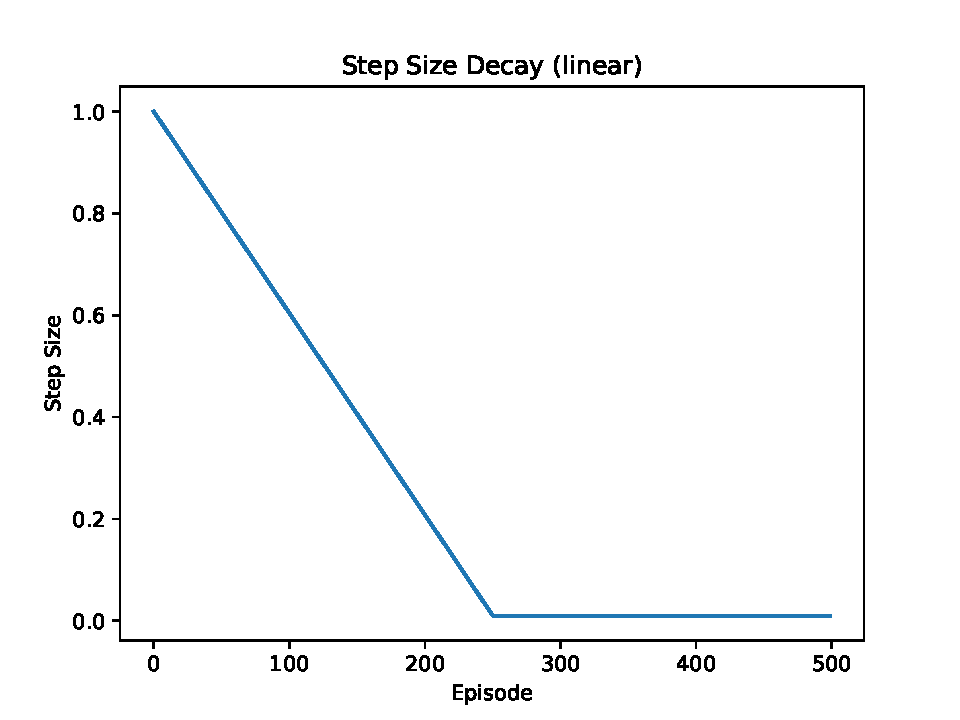
\includegraphics[width=0.8\textwidth]{images/mc_td/step_size_decay_linear.pdf}
        \caption{Exponential decay of step size}
        \label{fig:linear_step_size_decay}
    \end{figure}

    \item I implemented a routine to run Monte Carlo prediction for first-visit and every-visit scenarios. This is again controlled by \texttt{CONFIG} parameter. Below is an output from the routine for first-visit Monte Carlo prediction. The output consists of the state values, state-values for all episodes and the trajectory of the agent.
    \begin{verbatim}
(array([0., 0., 0., 0., 0., 0., 0.]),
array([[0., 0., 0., 0., 0., 0., 0.]]),
[(3, 0, 0.0, 2), (2, 0, 0.0, 1), (1, 0, 0.0, 0)])
    \end{verbatim}

    \item I implemented a routine to run Temporal difference prediction. This routine like the above not only does prediction but also computes the state-values. This is again controlled by \texttt{CONFIG} parameter. Below is an output from the routine for TD prediction routine. The output consists of the state values, state-values for all episodes and the trajectory of the agent.
    \begin{verbatim}
(array([0. , 0. , 0. , 0. , 0. , 0.1, 0. ]),
array([[0. , 0. , 0. , 0. , 0. , 0.1, 0. ]]),
[(3, 0, 0.0, 2), (2, 0, 0.0, 1), (1, 0, 0.0, 0)])
    \end{verbatim}
    \item I wrote a routine to plot the state-values across episodes and $log($episodes$)$ to answer multiple questions below. \texttt{plot\_episode\_values(V\_r, image\_name, config=None)} takes the state-values across episodes along with an \texttt{image\_name} to save the image and a \texttt{config} for additional information.

    I plotted the state-values for each state for First-Visit MC in Figure \ref{fig:default_fvmc} and \ref{fig:tuned_fvmc}. We can see from the from the figures that there is initially very high variance in the state-values but as the number of episodes increase the variance decreases and the state-values converge to the true values. The variance is higher in the default case as the step size is too high and the decay is too slow. The variance is lower in the tuned case as the step size is lower and the final value is also very low. On the log-scale plot, we can see that the state-values slowly rise towards the true values.

    \begin{figure}[h]
        \centering
        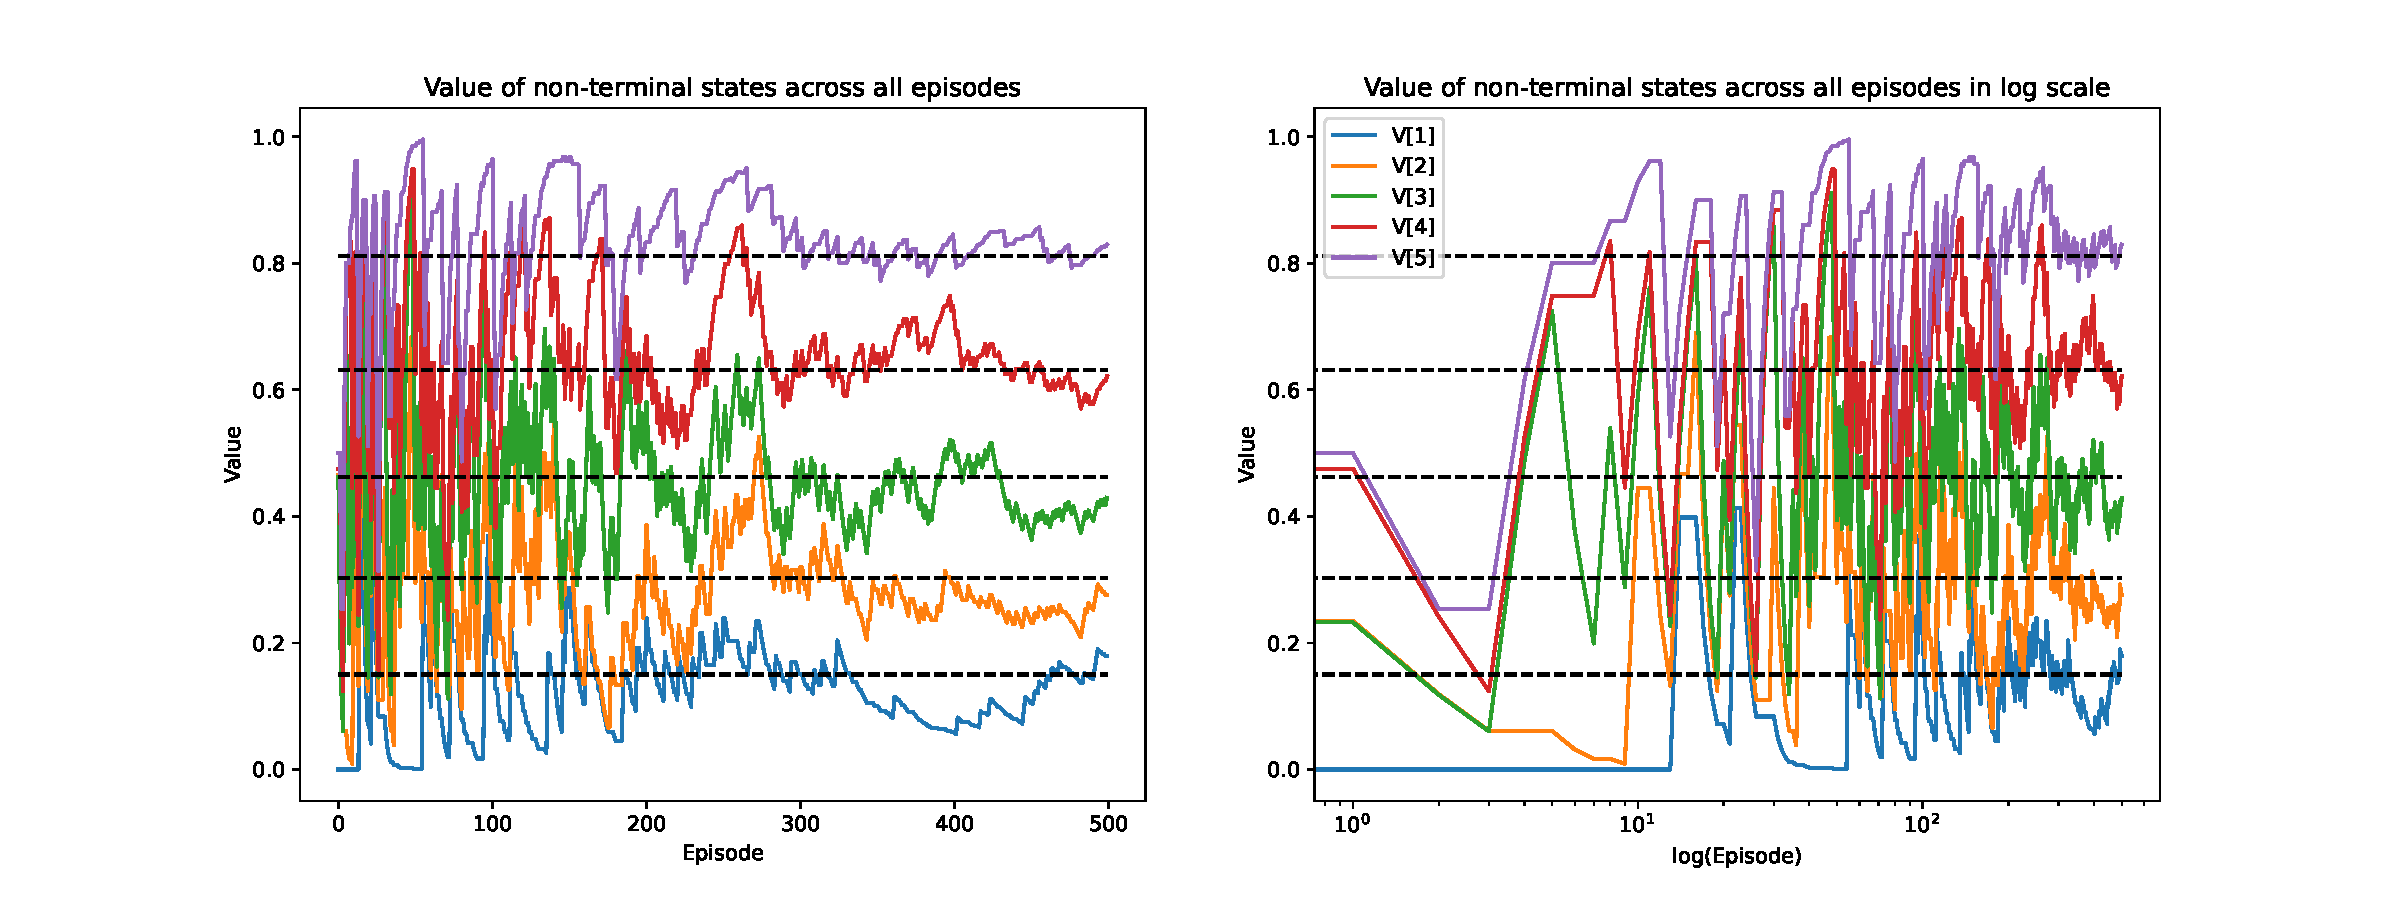
\includegraphics[width=\textwidth]{images/mc_td/first_visit_exponential_0.5_0.01_episode_values.pdf}
        \caption{FVMC with exponential decay of step size}
        \label{fig:default_fvmc}
    \end{figure}

    \begin{figure}[h]
        \centering
        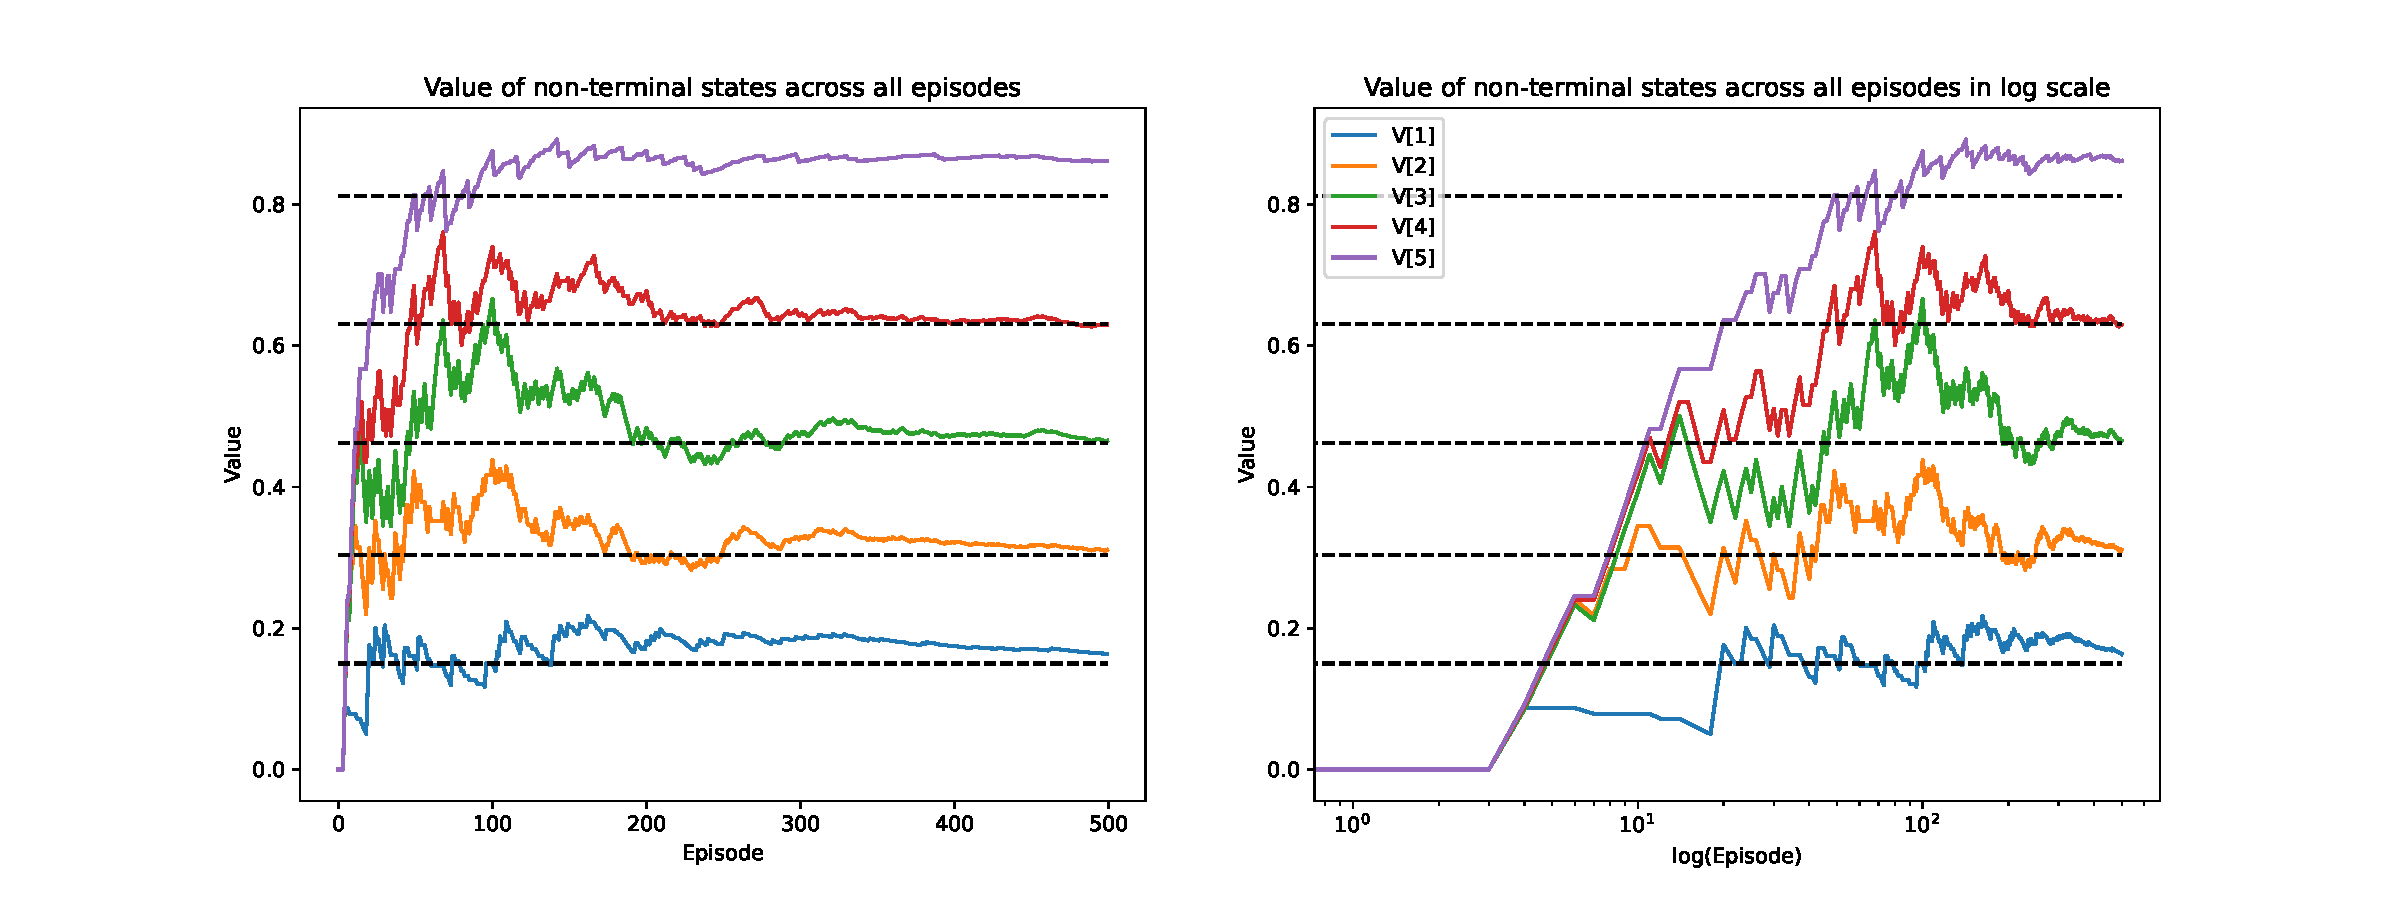
\includegraphics[width=\textwidth]{images/mc_td/first_visit_exponential_0.1_0.0008_episode_values.pdf}
        \caption{FVMC with exponential decay and tuned hyperparameters}
        \label{fig:tuned_fvmc}
    \end{figure}

    \item I plotted the state-values for each state for Every-Visit MC in Figure \ref{fig:default_evmc} and \ref{fig:tuned_evmc}. We can see from the from the figures that there is initially very high variance in the state-values but as the number of episodes increase the variance decreases and the state-values converge to the true values. The variance is higher in the default case as the step size is too high and the decay is too slow. I then tuned the hyperparameters and the variance is lower in the tuned case as the step size is lower and the final value is also very low, while achieving very low bias on the true values. On the log-scale plot, we can make a better judgement on the high variance phenomenon of Monte Carlo methods.
    \begin{figure}[h]
        \centering
        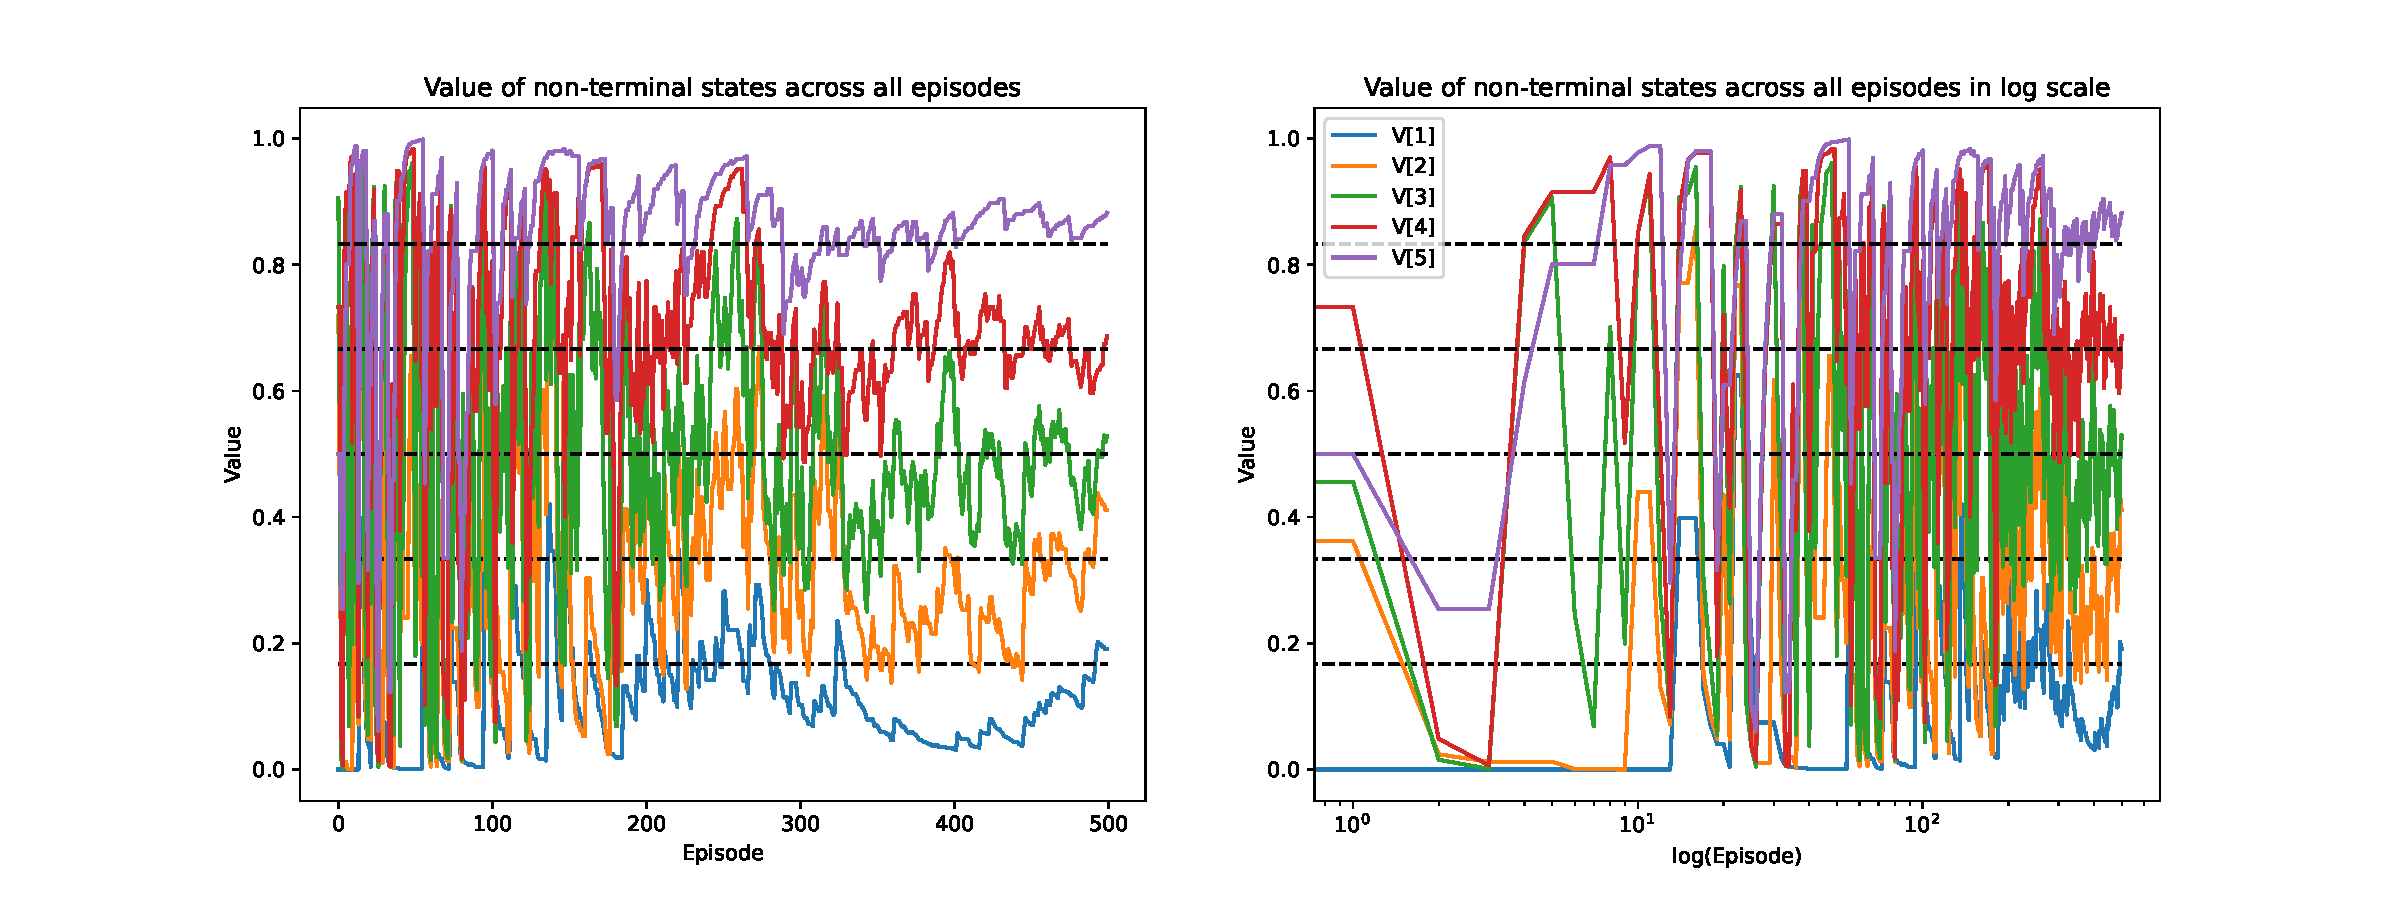
\includegraphics[width=\textwidth]{images/mc_td/every_visit_exponential_0.5_0.01_episode_values.pdf}
        \caption{EVMC with exponential decay of step size}
        \label{fig:default_evmc}
    \end{figure}

    \begin{figure}[h]
        \centering
        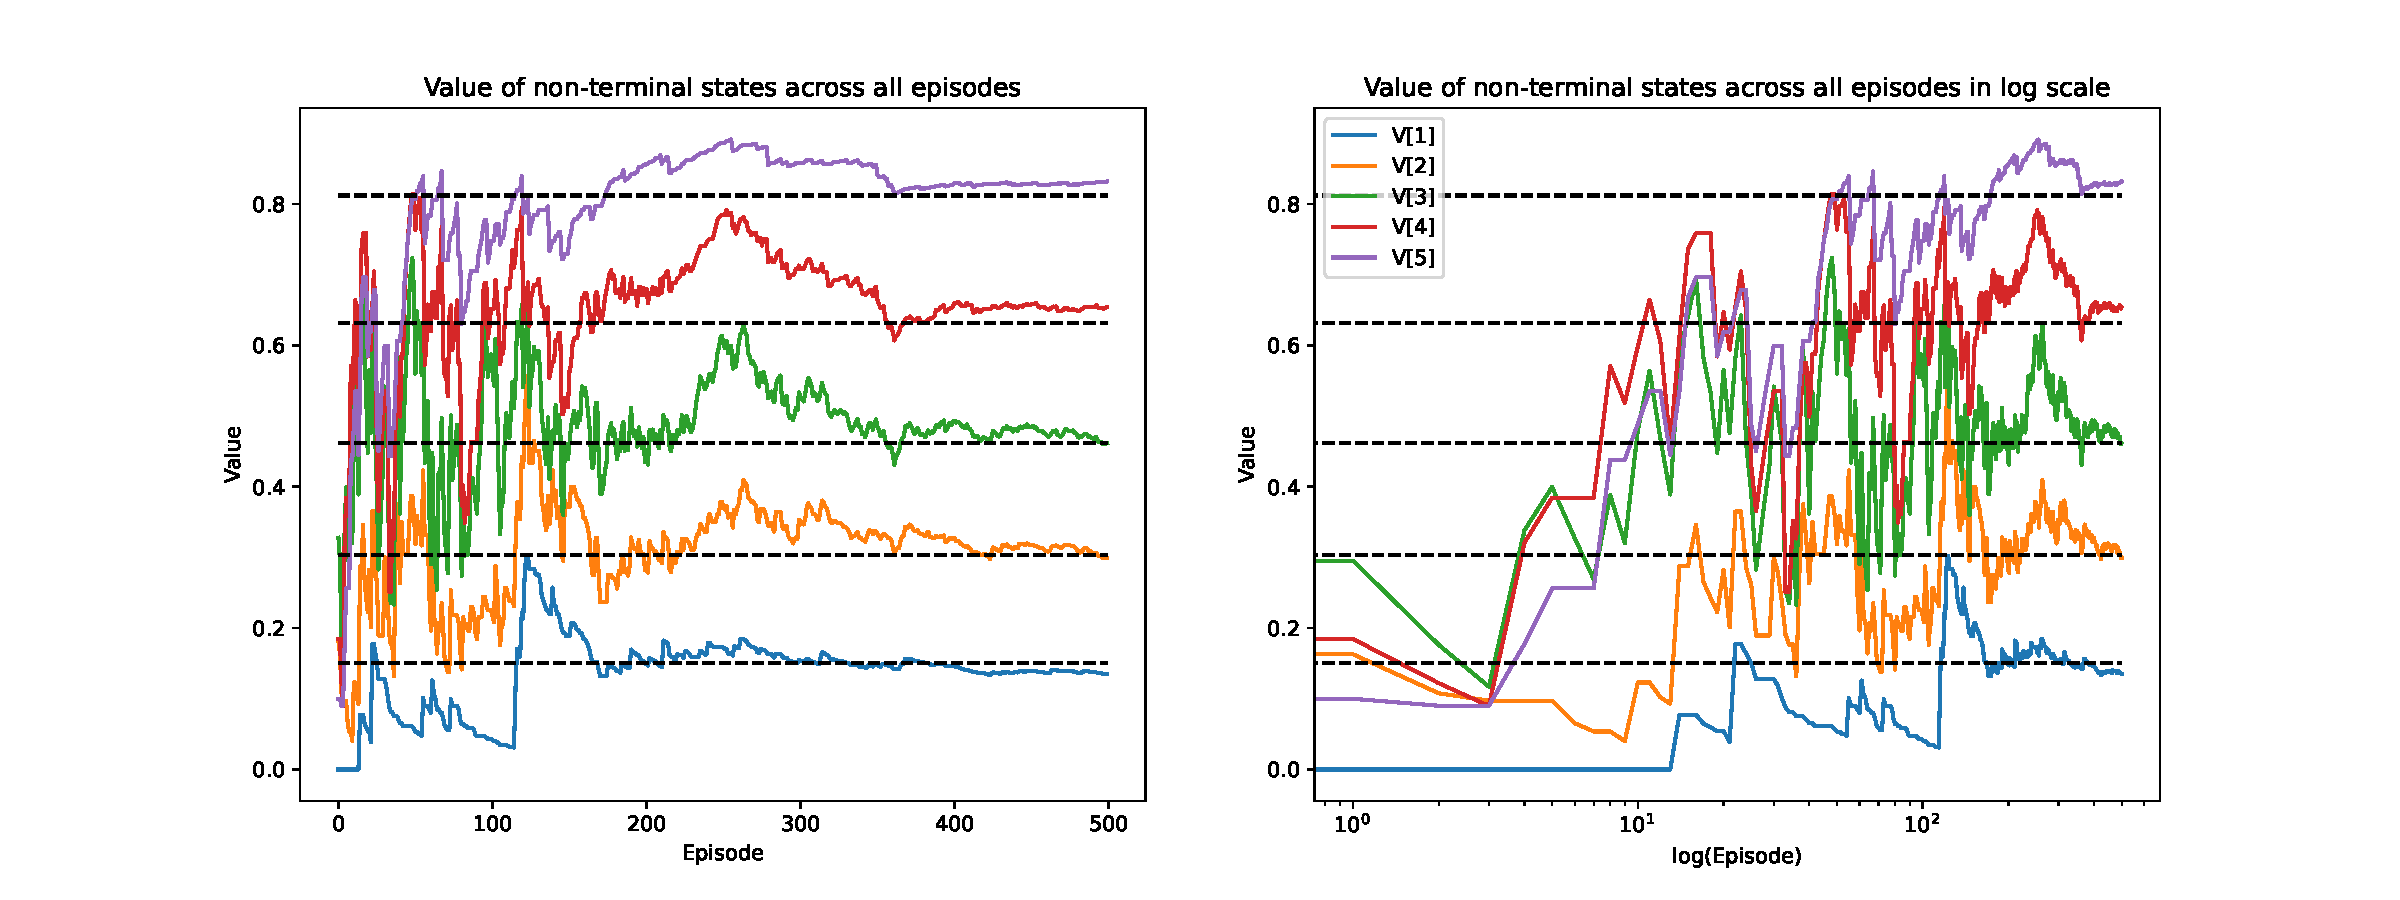
\includegraphics[width=\textwidth]{images/mc_td/every_visit_exponential_0.1_0.0008_episode_values.pdf}
        \caption{EVMC with exponential decay and tuned hyperparameters}
        \label{fig:tuned_evmc}
    \end{figure}

    \item I plotted the state-values for each state for TD prediction in Figure \ref{fig:default_td} and \ref{fig:tuned_td}. Before and after tuning we can observe that the variance in all the state-values of TD are low but the state-values never seem to converge at the true values. This shows the high bias TD learning has, as discussed in class.
    \begin{figure}[h]
        \centering
        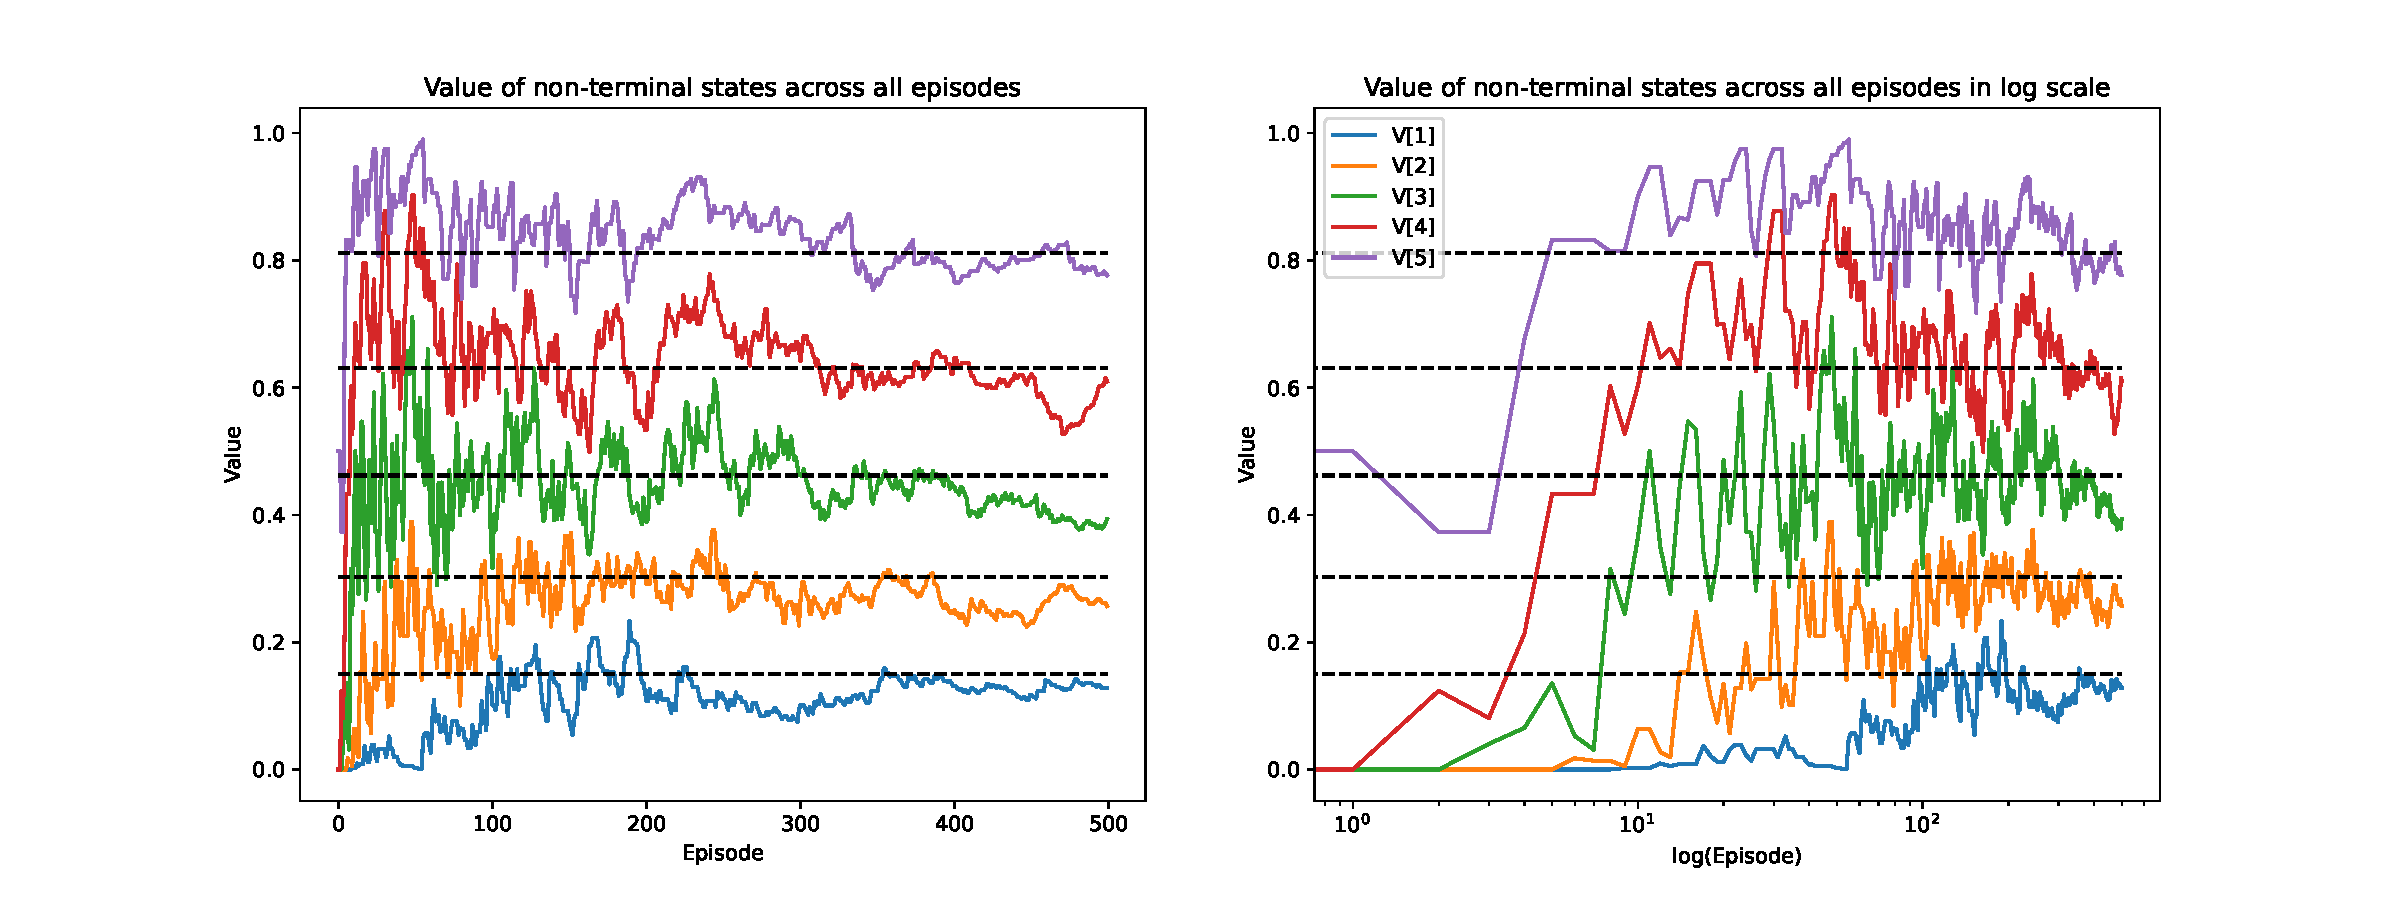
\includegraphics[width=\textwidth]{images/mc_td/td_learning_exponential_0.5_0.01_episode_values.pdf}
        \caption{TD with exponential decay of step size}
        \label{fig:default_td}
    \end{figure}

    \begin{figure}[h]
        \centering
        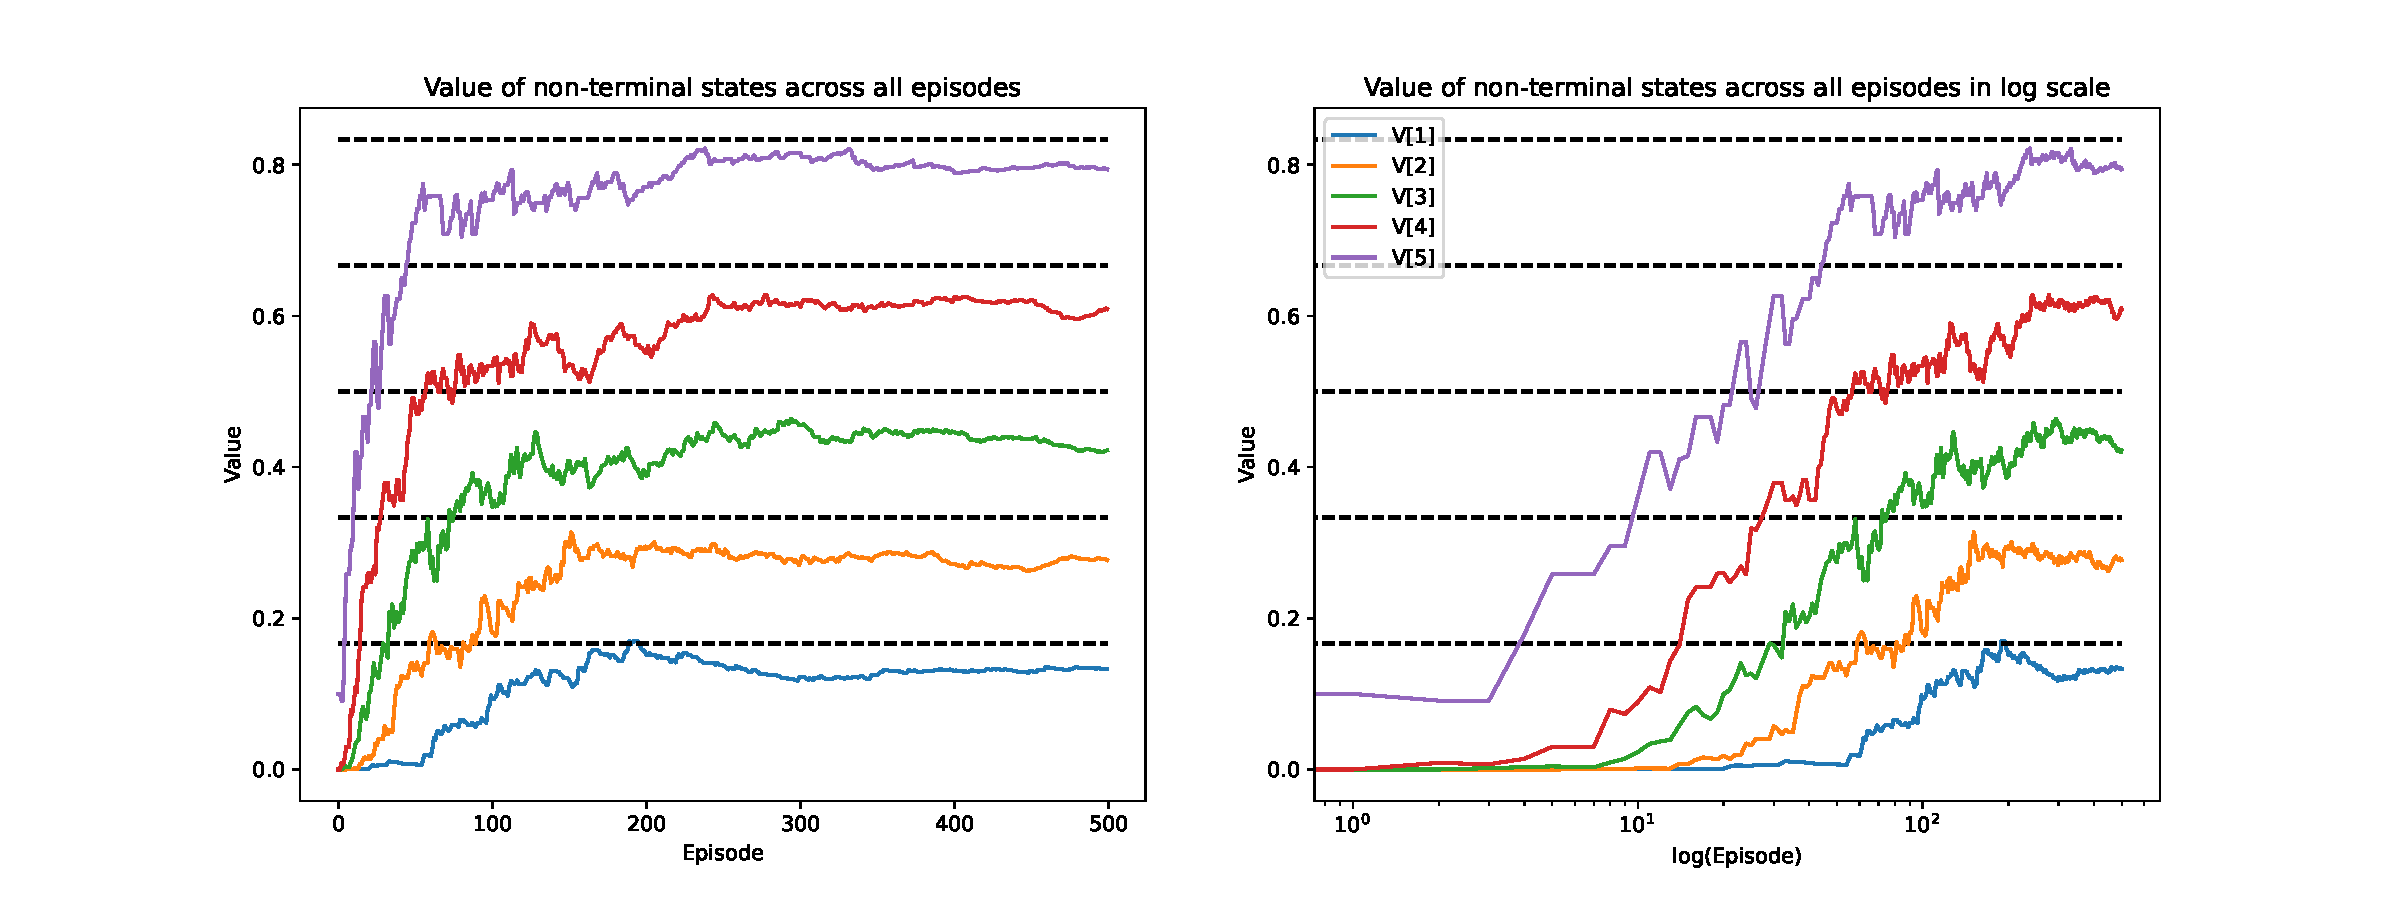
\includegraphics[width=\textwidth]{images/mc_td/td_learning_exponential_0.1_0.002_episode_values.pdf}
        \caption{TD with exponential decay and tuned hyperparameters}
        \label{fig:tuned_td}
    \end{figure}

    \item In this question I wrote a routine to run experiments for \texttt{max\_runs} number of times. The routine runs First-Visit MC, Every-Visit MC and TD learning for \texttt{max\_episodes} number of episodes using the tuned hyperparameters for each of the algorithms. The routine then plots the average state-values across all runs for each algorithm. The results are shown in Figure \ref{fig:average_fvmc}, \ref{fig:average_evmc} and \ref{fig:average_td}. We can see that the average state-values for First-Visit MC and Every-Visit MC converge to the true values but the average state-values for TD learning do not converge to the true values. This is consistent with the general behaviours of the algorithms.
    \begin{figure}[h]
        \centering
        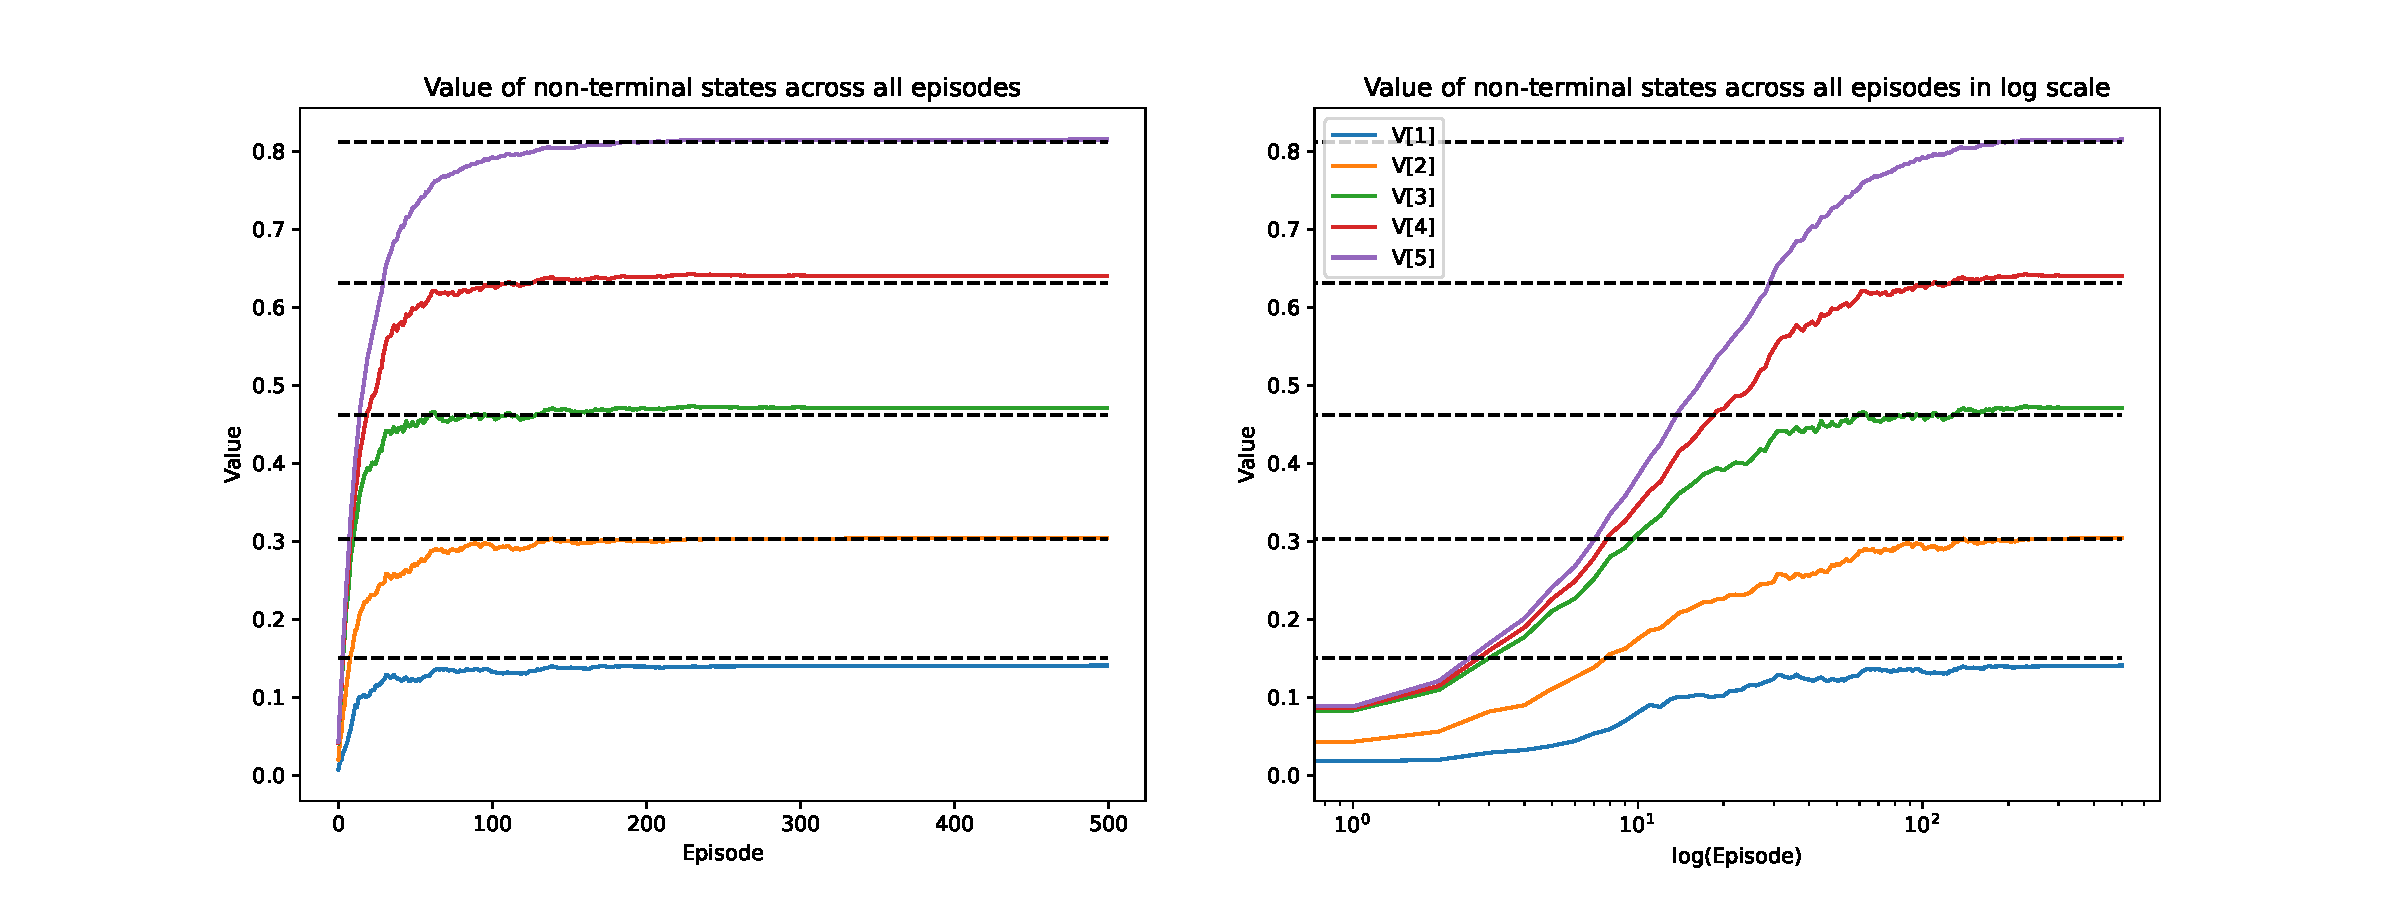
\includegraphics[width=\textwidth]{images/mc_td/fvmc_experiments_50.pdf}
        \caption{Average state-values of 50 runs of FVMC with exponential decay and tuned hyperparameters}
        \label{fig:average_fvmc}
    \end{figure}

    \begin{figure}[h]
        \centering
        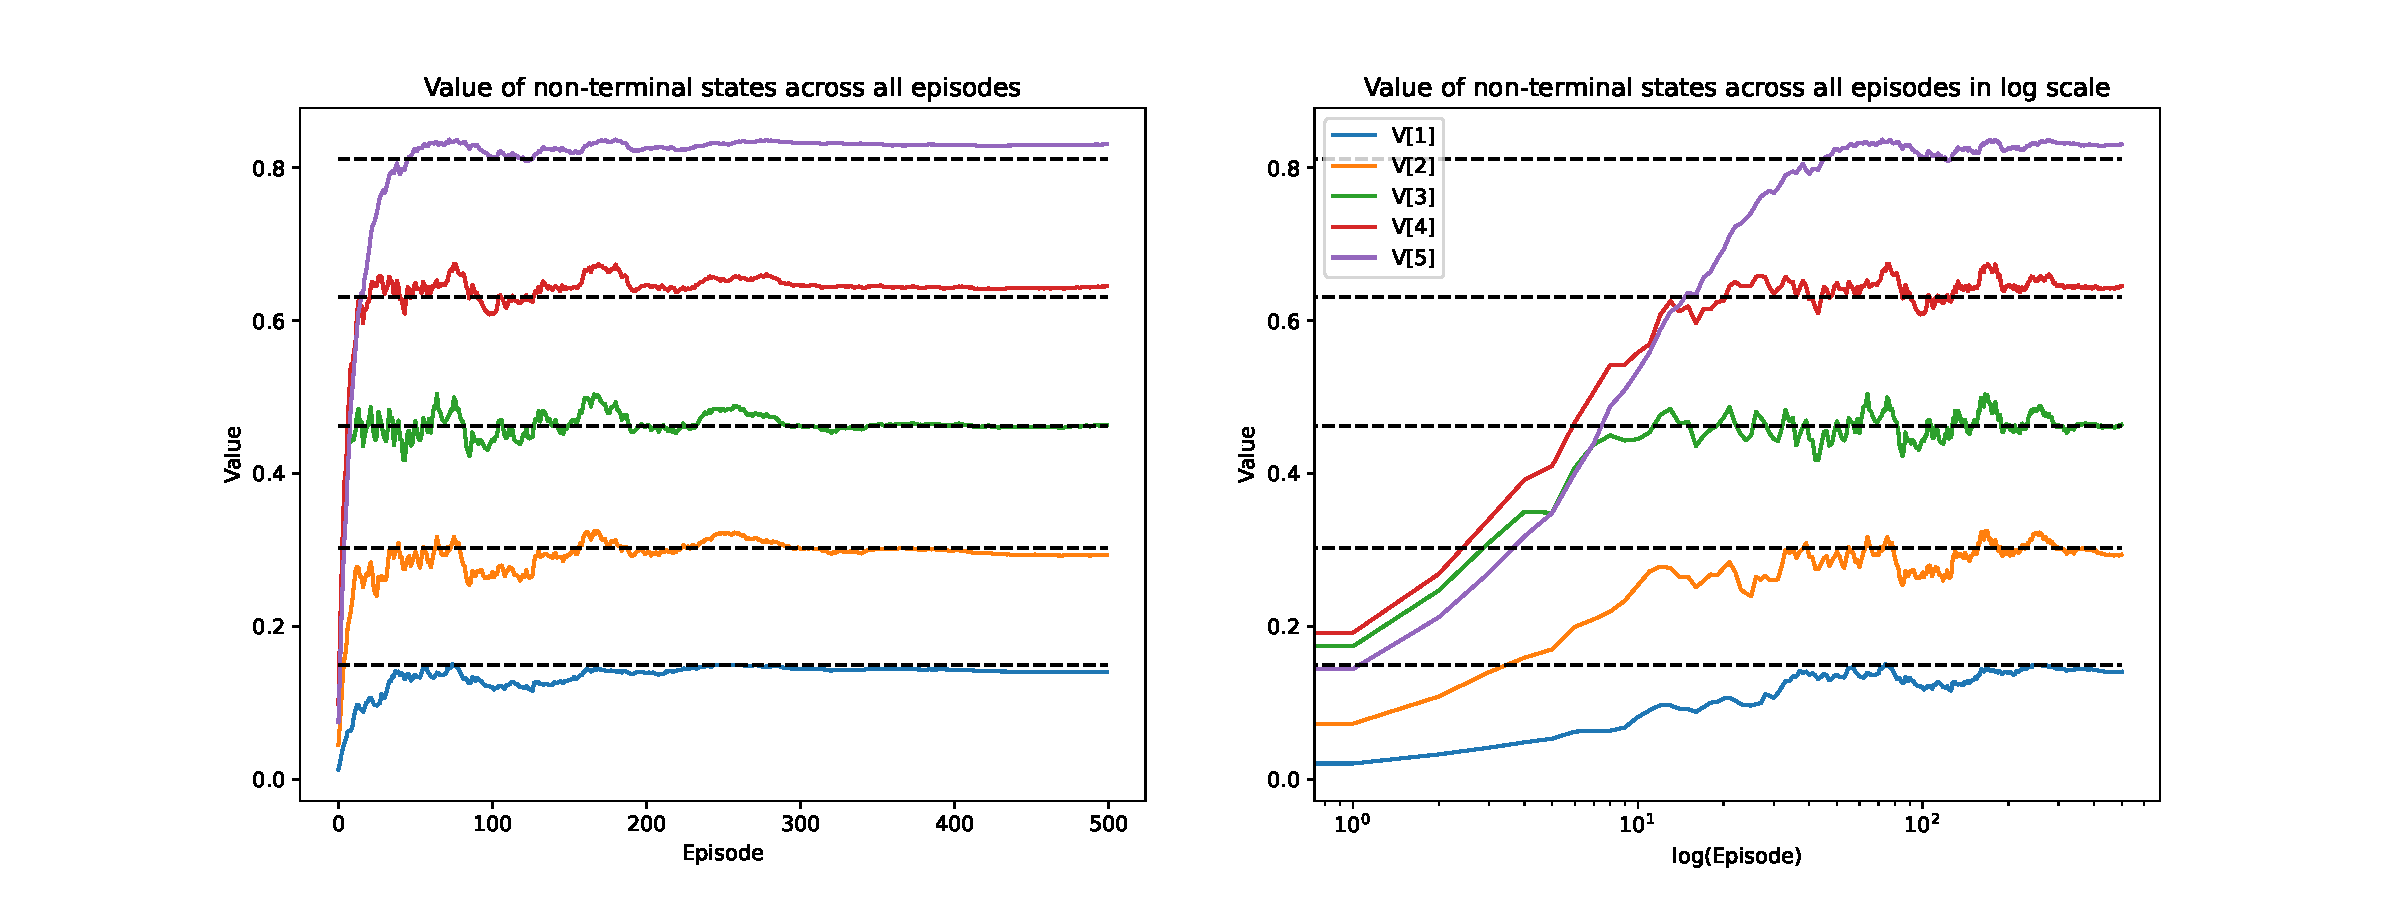
\includegraphics[width=\textwidth]{images/mc_td/evmc_experiments_50.pdf}
        \caption{Average state-values of 50 runs of EVMC with exponential decay and tuned hyperparameters}
        \label{fig:average_evmc}
    \end{figure}

    \begin{figure}[h]
        \centering
        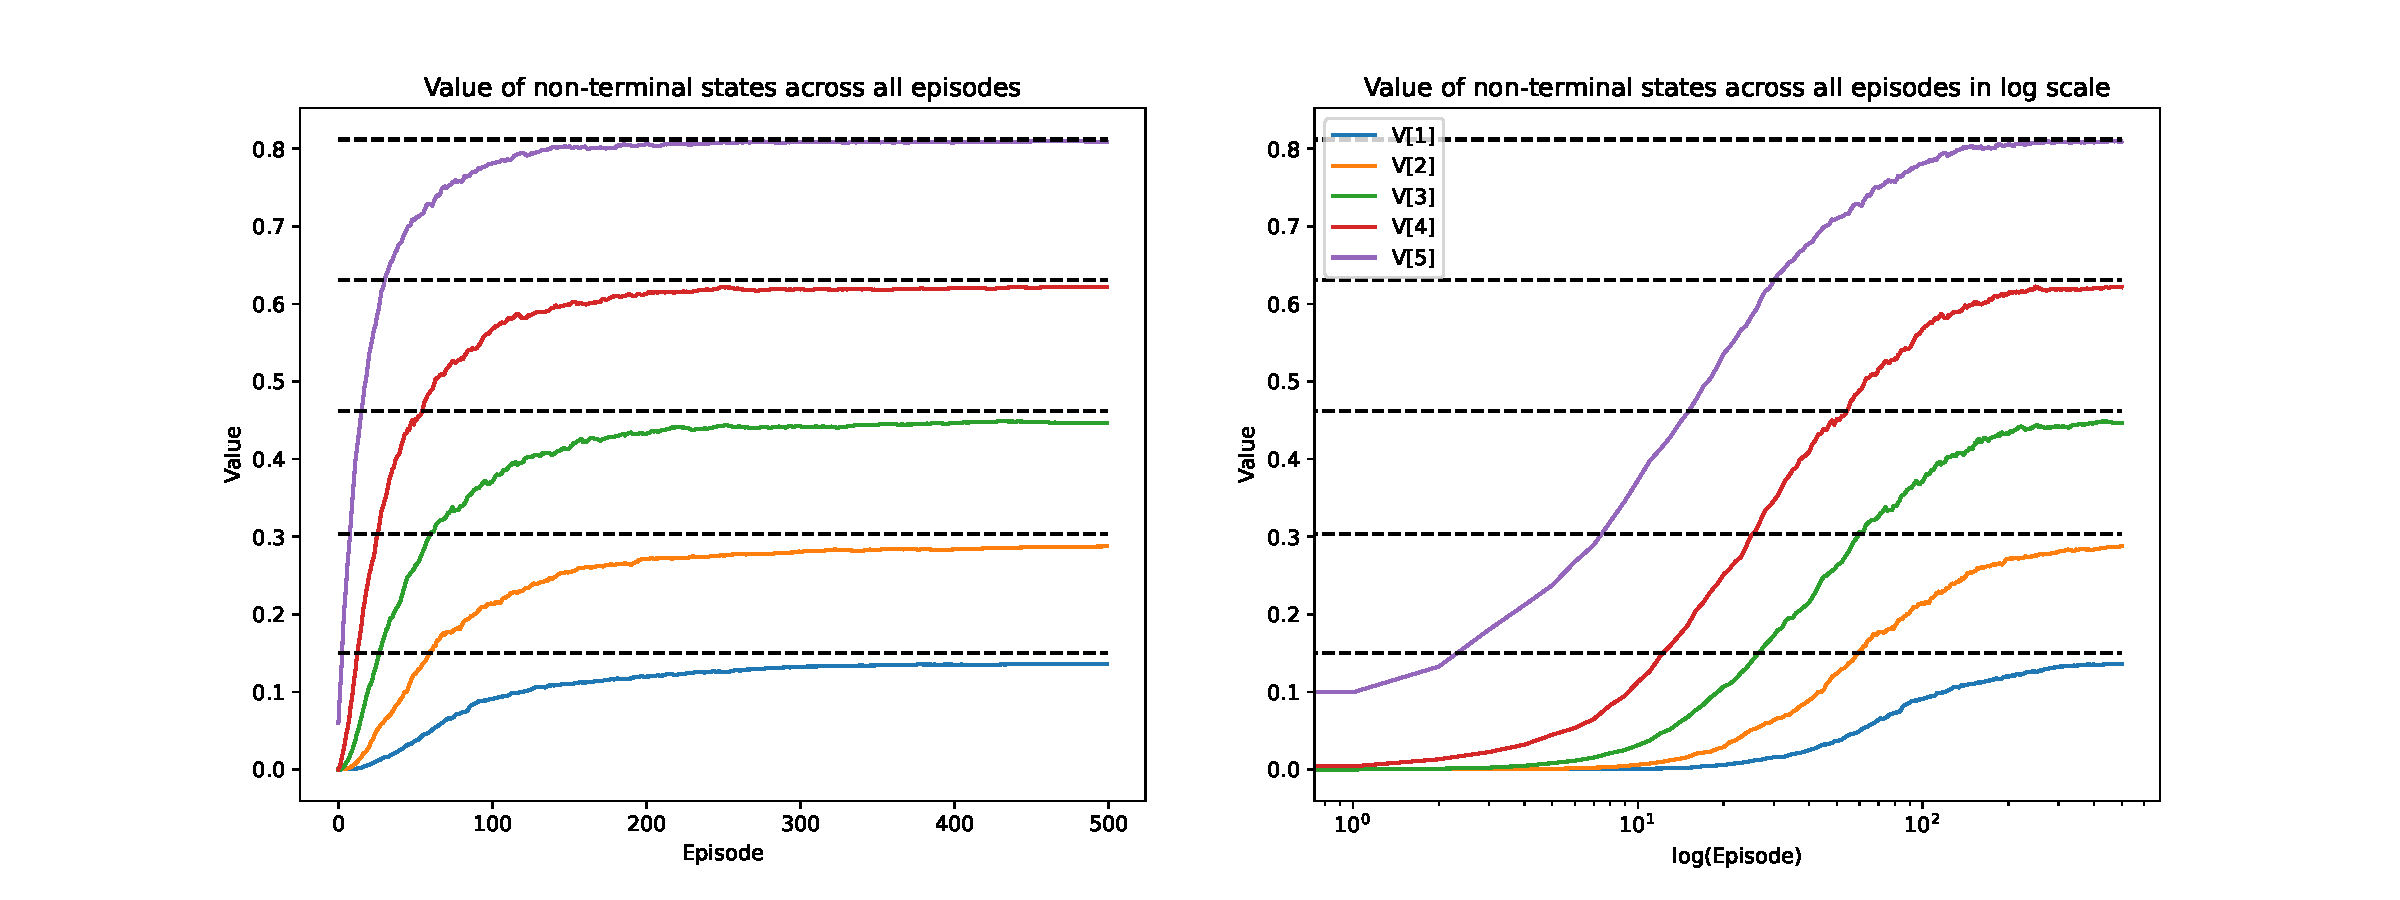
\includegraphics[width=\textwidth]{images/mc_td/td_experiments_50.pdf}
        \caption{Average state-values of 50 runs of TD with exponential decay and tuned hyperparameters}
        \label{fig:average_td}
    \end{figure}
    
    \item \textbf{Comparision of FVMC, EVMC and TD based on state-value functions across episodes and log-scale of episodes:} We can see that the state-values for FVMC and EVMC converge to the true values but the state-values for TD learning do not converge to the true values. This is consistent with the general behaviours of the algorithms. The variance in the state-values for FVMC and EVMC is higher than TD learning but the bias in the state-values for TD learning is higher than FVMC and EVMC. The plot on log-scale helps us to zoom into the first few episodes and make a better judgement on the high variance phenomenon of Monte Carlo methods.
    \item \textbf{Comparision of FVMC, EVMC and TD based on average target value for state 3:} We can see that the average across episodes for FVMC and EVMC osciilates between 0 and 1 but the average for TD learning has fewer oscillations but does not land at the true values. Thus, this is another view to note the high variance in Monte Carlo methods and the high bias in TD learning.

\end{enumerate}